\section{Experiments}

We evaluated the proposed approach on a suite of 55 Atari 2600 games.\footnote{
Code available at \url{https://github.com/fred5577/VAE-IW}}
%
We separately trained a VAE for each domain by maximizing~\cref{eq:beta_objective_function} using stochastic gradient ascent.
%
To train the VAEs, we collected 15,000 frames by running RolloutIW(1) with B-PROST features, and split them into a training and validation set of 14,250 and 750 images.

The encoder consists of 3 convolutional layers interleaved with residual blocks. The single convolutional layers downsample the feature map by a factor of 2, and each residual block includes 2 convolutional layers, resulting in 7 convolutional layers in total. The decoder mirrors such architecture, and uses transposed convolutions for upsampling. Further architectural details are provided in the Appendix.
The inference network outputs a feature map of shape $H \times W \times C$ which represents the approximate posterior probabilities of the latent variables. Thus, unlike traditional VAEs where latent variables do not carry any spatial meaning, in our case they are spatially arranged~\cite{vahdat2020nvae}.

As outlined in the previous section, the Bernoulli probabilities computed by the encoder are thresholded, and the resulting binary features are used as propositional representations for planning in RolloutIW(1), instead of the B-PROST features.
For the planning phase of VAE-IW(1), we use RolloutIW(1) with partial caching and risk aversion (RA) as described by \citet{rolloutiw-orginal}. With partial caching, after each iteration of RolloutIW(1), the branch of the chosen action is kept in memory. Risk aversion is attained by multiplying all negative rewards by a factor $\alpha \gg 1$ when they are propagated up the tree.

Because of their diversity, Atari games vary widely in complexity.
We empirically chose a set of hyperparameters that performed reasonably well on a small subset of the games, assuming this would generalize well enough to other games.
Following previous work~\cite{iworginal,rolloutiw-orginal}, we used a frame skip of 15 and a planning budget of 0.5s per time step.
We set an additional limit of 15,000 executed actions for each run, to prevent runs from lasting too long (note that this constraint is only applied to our method).
We expect that better results can be obtained by performing an extensive hyperparameter search on the whole Atari suite.
See the Appendix for further implementation details.


\subsection{Main Results}


\begin{table}[!t]
    \centering
    \begin{minipage}{\columnwidth}
    \resizebox{\columnwidth}{!}{%
\begin{tabular}{lrrrrrrrl}

\toprule
% Algorithm& Human & IW &  RA RolloutIW & RA VAE-IW \\
% Features& & B-PROST & B-PROST & VAE $15 \times 15 \times 20$\\
% Planning budget& & 0.5s & 0.5s &  0.5s  \\
Algorithm & Human & IW &  RolloutIW & VAE-IW \\
 Features & & B-PROST &  B-PROST & VAE \\

\midrule
Alien            & 6,875                & 1,316          & 7,170           & \textbf{7,744}     \\
Amidar           & 1,676                & 48             & 1,049.2           & \textbf{1,380.3}     \\
Assault          & 1,496                & 268.8            & 336             & \textbf{1,291.9}     \\
Asterix          & 8,503                & 1,350          & 46,100          & \textbf{999,500*}   \\
Asteroids        & 13,157               & 840            & 4,698           & \textbf{12,647}    \\
Atlantis         & 29,028               & 33,160         & 122,220         & \textbf{1,977,520*} \\
BankHeist        & 734.4                   & 24             & 242             & \textbf{289}       \\
BattleZone       & 37,800               & 6,800          & 74,600          & \textbf{115,400}   \\
BeamRider        & 5,775                & 715.2            & 2,552.8           & \textbf{3,792}     \\
Berzerk          & \multicolumn{1}{l}{} & 280            & \textbf{1,208}  & 863                \\
Bowling          & 154.8                   & 30.6             & 44.2              & \textbf{54.4}        \\
Boxing           & 4.3                     & \textbf{99.4}    & 99.2              & 89.9                 \\
Breakout         & 31.8                    & 1.6              & \textbf{86.2}     & 45.7                 \\
Centipede        & 11,963               & 88,890         & 56,328          & \textbf{428,451.5*}   \\
ChopperCommand   & 9,882                & 1,760          & \textbf{9,820}  & 4,190              \\
CrazyClimber     & 35,411               & 16,780         & 40,440          & \textbf{901,930*}   \\
DemonAttack      & 3,401                & 106            & 6,958           & \textbf{285,867.5*}   \\
DoubleDunk       & -15.5                   & -22            & 3.2               & \textbf{8.6}         \\
ElevatorAction   & \multicolumn{1}{l}{} & 1,080          & 0               & \textbf{40,000*}    \\
Enduro           & 309.6                   & 2.6              & \textbf{145.8}    & 55.5                 \\
FishingDerby     & 5.5                     & -83.8            & -77             & \textbf{-20}       \\
Freeway          & 29.6                    & 0.6              & 2               & \textbf{5.3}         \\
Frostbite        & 4,335                & 106            & 146             & \textbf{259}       \\
Gopher           & 2,321                & 1,036          & 8,388           & \textbf{8,484}     \\
Gravitar         & 2,672                & 380            & 1,660           & \textbf{1,940}     \\
IceHockey        & 0.9                     & -13.6            & -12.4             & \textbf{37.2}        \\
Jamesbond        & 406.7                   & 40             & \textbf{10,760} & 3,035              \\
Kangaroo         & 3,035                & 160            & \textbf{1,880}  & 1,360              \\
Krull            & 2,395                & 3,206.8          & 2,091.8           & \textbf{3,433.9}     \\
KungFuMaster     & 22,736               & 440            & 2,620           & \textbf{4,550}     \\
MontezumaRevenge & 4,367                & 0              & \textbf{100}    & 0                  \\
MsPacman         & 15,693               & 2,578          & 15,115          & \textbf{17,929.8}    \\
NameThisGame     & 4,076                & 7,070          & 6,558           & \textbf{17,374}    \\
Phoenix          & \multicolumn{1}{l}{} & 1,266          & \textbf{6,790}  & 5,919              \\
Pitfall          & \multicolumn{1}{l}{} & -8.6             & -302.8            & \textbf{-5.6}        \\
Pong             & 9.3                     & -20.8            & -4.2              & \textbf{4.2}         \\
PrivateEye       & 69,571               & \textbf{2,690.8} & -480            & 80                 \\
Qbert            & 13,455               & 515            & \textbf{15,970} & 3,392.5              \\
Riverraid        & 13,513               & 664            & 6,288           & \textbf{6,701}     \\
RoadRunner       & 7,845                & 200            & \textbf{31,140} & 2,980              \\
Robotank         & 11.9                    & 3.2              & \textbf{31.2}     & 25.6                 \\
Seaquest         & 20,182               & 168            & \textbf{2,312}  & 842                \\
Skiing           & \multicolumn{1}{l}{} & -16,511        & -16,006.8         & \textbf{-10,046.9}   \\
Solaris          & \multicolumn{1}{l}{} & 1,356          & 1,704           & \textbf{7,838}     \\
SpaceInvaders    & 1,652                & 280            & 1,149           & \textbf{2,574}     \\
StarGunner       & 10,250               & 840            & \textbf{14,900} & 1,030              \\
Tennis           & -8.9                    & -23.4            & -5.4              & \textbf{4.1}         \\
TimePilot        & 5,925                & 2,360          & 3,540           & \textbf{32,840}    \\
Tutankham        & 167.7                   & 71.2             & 135.6             & \textbf{177}       \\
UpNDown          & 9,082                & 928            & 34,668          & \textbf{762,453*}   \\
Venture          & 1,188                & 0              & \textbf{60}     & 0                  \\
VideoPinball     & 17,298               & 28,706.4         & 216,468.6         & \textbf{373,914.3}   \\
WizardOfWor      & 4,757                & 5,660          & 43,860          & \textbf{199,900}   \\
YarsRevenge      & \multicolumn{1}{l}{} & 6,352.6          & 7,848.8           & \textbf{96,053.3}    \\
Zaxxon           & 9,173                & 0              & 15,500          & \textbf{15,560}    \\
\midrule
\# $>$ Human  & n/a  & 4 & 22 & 25  \\
\# $>$ 75\% Human  & n/a  & 4 & 26 & 28  \\
\midrule
\# best in game & n/a & 2 & 14 &  39 \\
\bottomrule
\end{tabular}%
}
% \end{center}
\caption{Score comparison in 55 Atari games. Scores in bold indicate the best width-based method, and a star indicates that the limit on executed actions was reached at least once. 
RolloutIW and VAE-IW are run with risk aversion.
%In the bottom rows we also report the number of domains in which an algorithm's score was greater than the human score, or greater than $\%75$ of the human score. 
% Human scores are from \citet{liang}.
% Results for IW and Rollout IW B-PROST are from \citet{rolloutiw-orginal}; human scores are from \citet{liang}.
} 
\label{tab:atari-lookahead-0.5}

    \end{minipage}
\end{table}

\begin{figure*}[!ht]
    \centering
    % \includegraphics[width=\paperwidth]{Pictures/final_normalized_scores_v2xcf.png}
    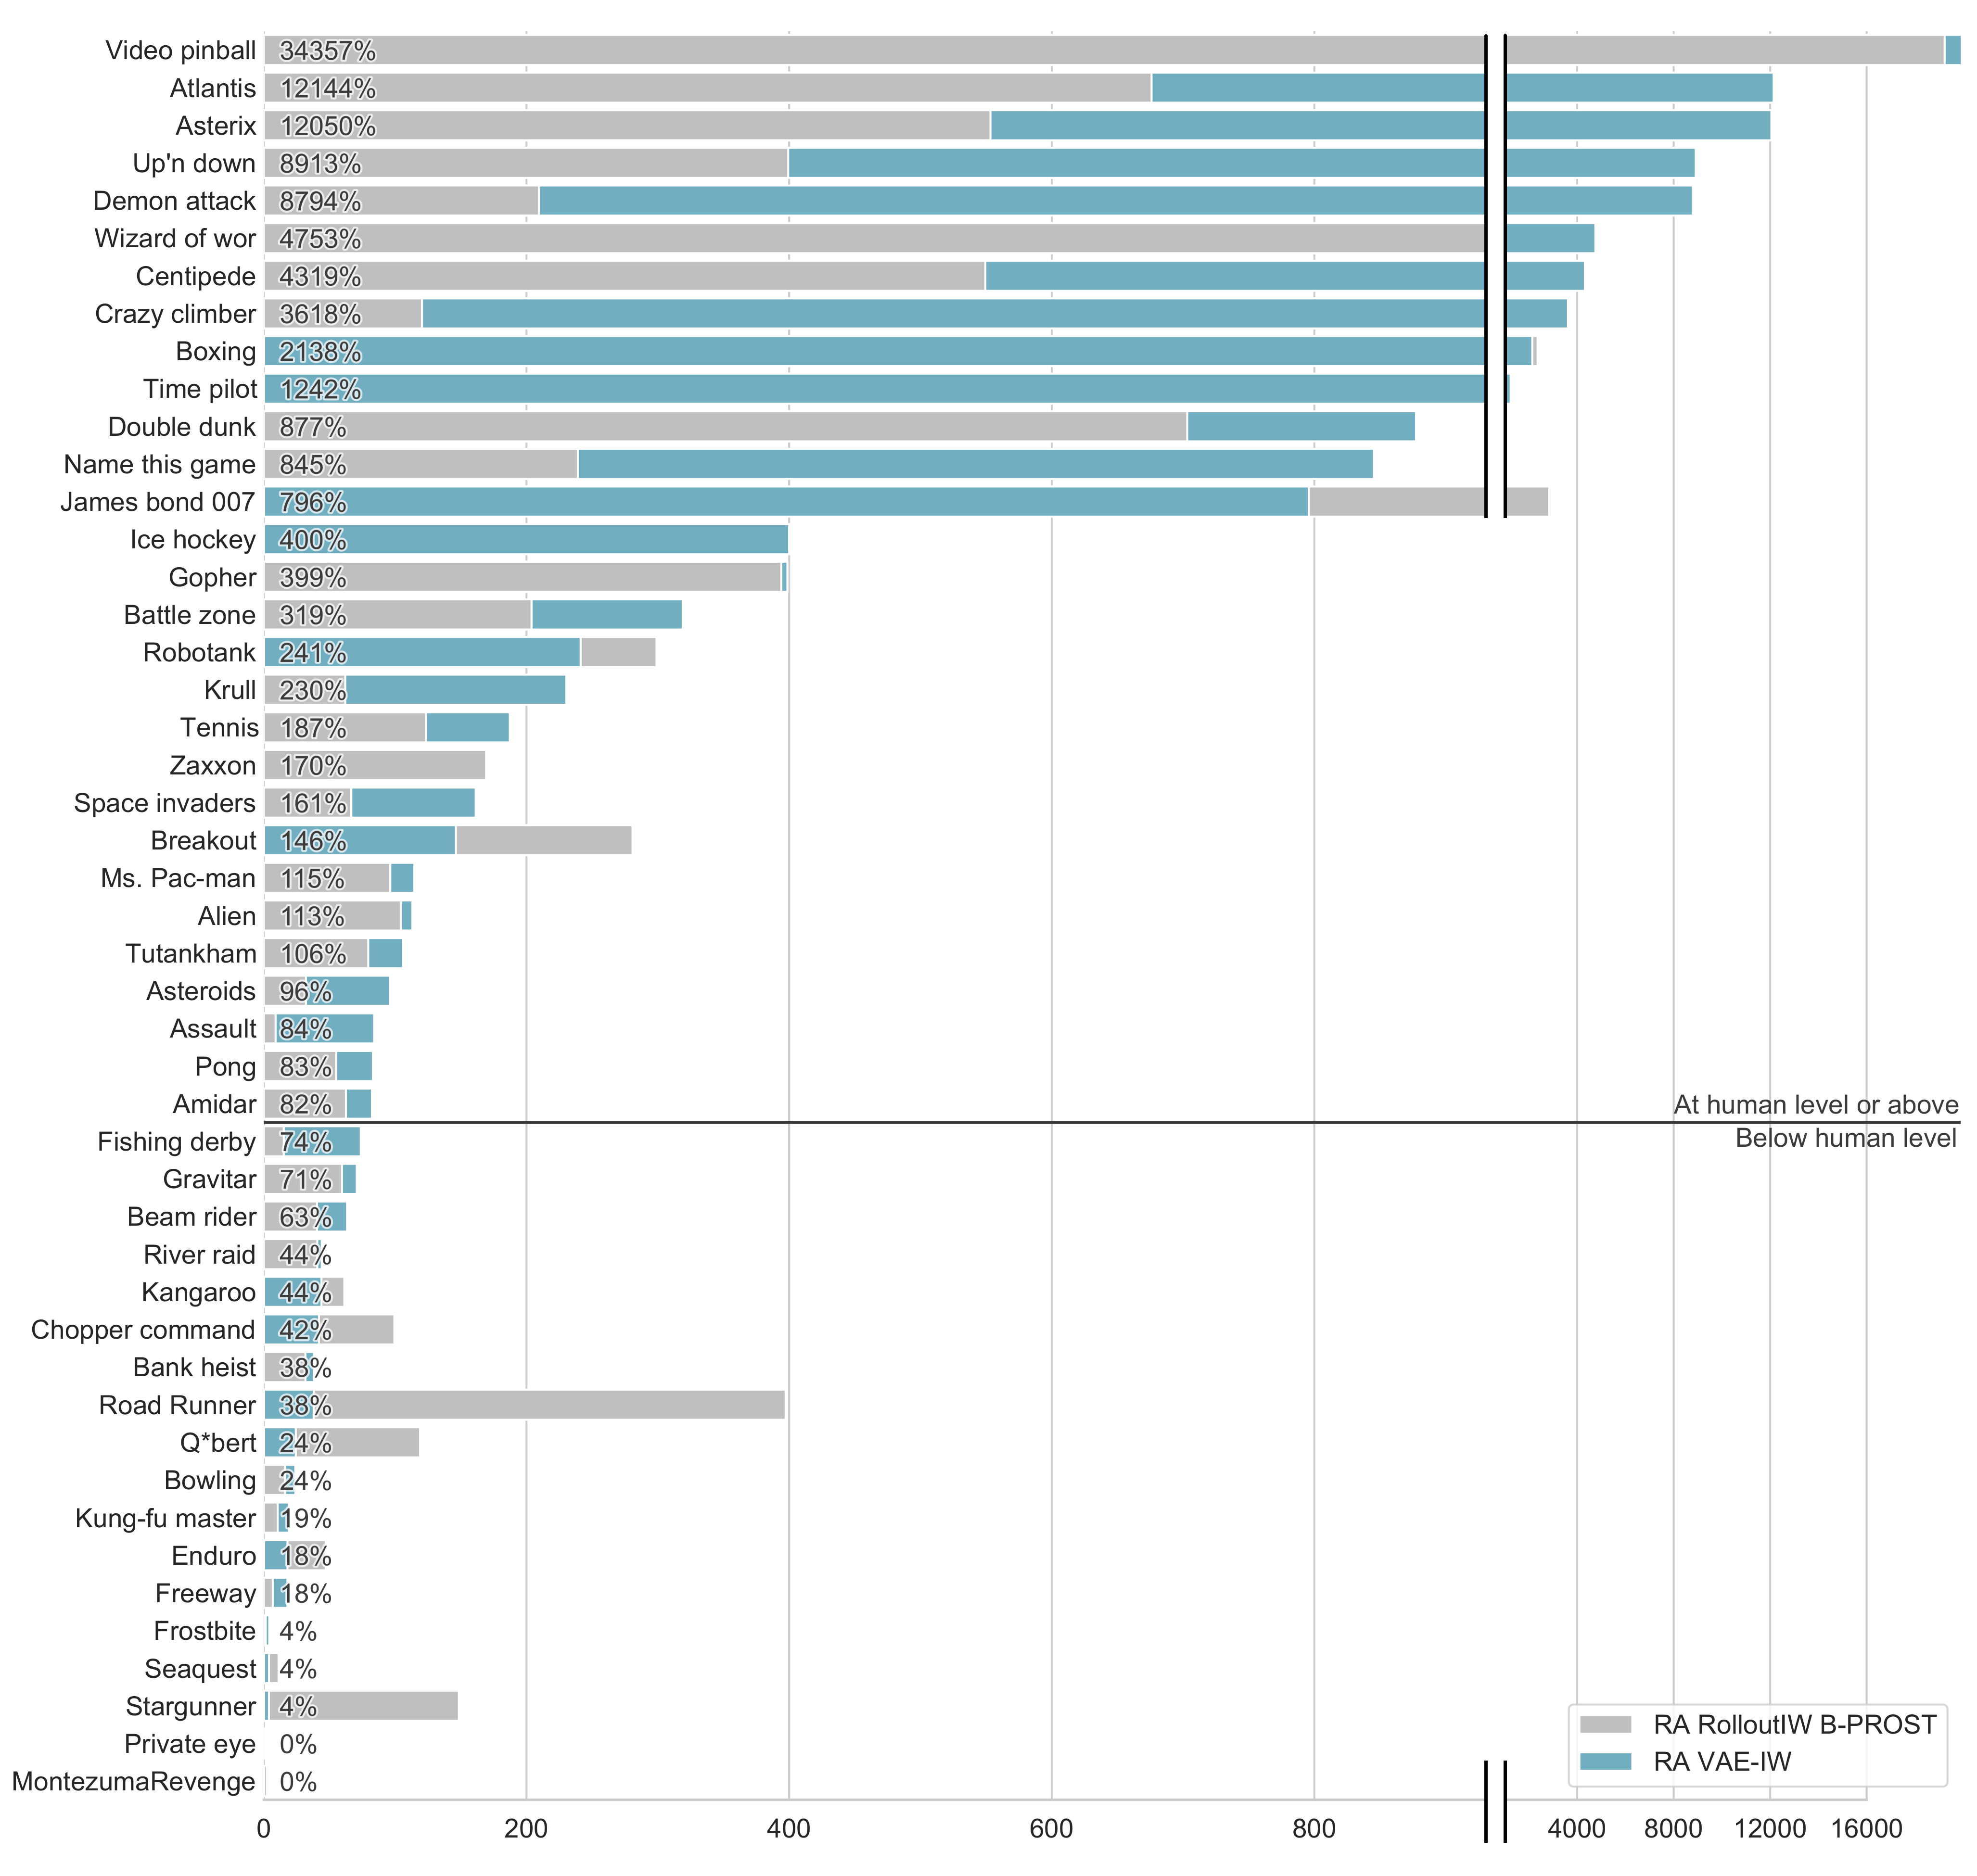
\includegraphics[width=\textwidth]{Pictures/big-plot-v2.png}
    \caption{Comparison of the risk-averse variants of VAE-IW(1) (ours, using {VAE} features) and RolloutIW(1) B-PROST (using {B-PROST} features). Following \citet{minh}, the performance of both methods is normalized with respect to a professional human game tester (100\% level) and random play (0\%) as: $100 \times (
    \text{VAE}-\text{random play})/(\text{human score}-\text{random play})$. RA VAE-IW(1) obtains the highest score among width-based approaches in most games, and it performs at a level that is superior to or comparable with professional human play. The reported percentages are for VAE features.}
    \label{fig:cool_plot}
\end{figure*}


In Table~\ref{tab:atari-lookahead-0.5}, we compare the planning performance of our RA VAE-IW(1) to IW(1) with B-PROST features, RA RolloutIW(1) with B-PROST features, and human play \citep{liang}. 
In Figure~\ref{fig:cool_plot}, we normalize the scores of width-based planning methods using scores from random and human play, as in \citet{rolloutiw-orginal}. Note that human play is only meant as a baseline: since humans do not have access to a simulator, a direct comparison cannot be made. 
Following the literature, we report the average score over 10 runs, with each run ending when the game is over.
%
These results show that learning features purely from images, without any supervision, can be beneficial for width-based planning. In particular, using the learned representations in RolloutIW(1) leads to generally higher scores in the Atari 2600 domain. 
%
For reference, in \cref{tab:atari-piiw-rainbow} we provide an additional comparison of our method with other related approaches. However, these significantly differ from VAE-IW in some aspects and are therefore not directly comparable.

Note that the performance of VAE-IW depends on the quality and expressiveness of the features extracted by the VAE, which in turn depend on the images the VAE is trained on. Crucially, since we collect data by running RolloutIW with B-PROST features, the performance of VAE-IW is constrained by the effectiveness of the data collection algorithm. The VAE features will not necessarily be meaningful on parts of the game that are significantly different from those in the training set. Surprisingly, however, our method significantly outperforms the baseline that was used for data collection, providing even stronger evidence that the compact set of features learned by a VAE can be successfully utilized in width-based planning.
This form of bootstrapping can be iterated: images collected by VAE-IW could be used for re-training or fine-tuning VAEs, potentially leading to further performance improvements. Although in principle the first iteration of VAEs could be trained from images collected via random play, this is not a viable solution in hard-exploration problems such as many Atari games \cite{ecoffet2019go}.

In addition, there appears to be a significant negative correlation between the average number of true features and the average number of expanded nodes per planning phase (Spearman rank correlation of $-0.51$, p-value $< 0.001$). In other words, in domains where the VAE extracts on average more true features, the planning algorithm tends to expand fewer nodes. Thus, it could be potentially fruitful to further investigate the interplay between the average number of true features, the meaningfulness and usefulness of the features, and the efficiency of the width-based planning algorithm.


\subsection{Ablation Studies}

The performance of VAE-IW depends on hyperparameters of the planning algorithm and the probabilistic model.  Here we investigate the effect of some of these parameters. Tables with full results are reported in the Appendix.

\paragraph{Modeling choices.}

One of the major modeling choices is the dimensionality of the latent space, and the spatial structure $H \times W \times C$ of the latent variables. Both of these factors are tightly coupled with the neural architecture underlying the inference and generative networks. As there is no clear heuristic, we explored different neural architectures and latent space sizes. Based on the performance on a few selected domains, we chose two representative settings, with latent space size $15 \times 15 \times 20$ and $4 \times 4 \times 200$ (see the Appendix for further details). In Table~\ref{tab:atari-model-comp} we compare the performance of RA VAE-IW(1) on these two configurations, keeping the rest of the hyperparameters fixed as the ones used in Table~\ref{tab:atari-lookahead-0.5}. While overall the $15 \times 15 \times 20$ configuration leads to a higher score in most domains, the effect of this modeling choice seems to significantly depend on the domain.

An alternative to directly training a discrete latent variable model is to train a continuous one and then quantize the inferred representations at planning time. We investigated this possibility by training a continuous VAE with latent space size $15 \times 15 \times 5$ and independent prior $\mathcal{N}(0, 1)$ for each latent variable. When planning, we quantize the inferred posterior means into $2^4$ or $2^6$ bins of equal probability under the prior. This leads to 4 or 6 bits per latent variable, and hence 4,500 and 6,750 boolean features, respectively. In Table~\ref{tab:continuous}, we observe that this approach, although generally competitive, tends to be inferior to training a discrete model directly.

As previously mentioned, we consider the framework of $\beta$-VAEs in which $\beta$ controls the trade-off between the reconstruction accuracy and the amount of information encoded in the latent space. For our purposes, $\beta$ has to be small enough that the model can capture all relevant details in an image. In practice, we decreased $\beta$ until the model generated sufficiently accurate reconstructions on a selection of Atari games. Table~\ref{tab:atari-comparison} reports the performance of VAE-IW(1) when varying $\beta \in \{10^{-4}, 10^{-3}\}$, and shows that the effect of varying $\beta$ depends on the domain. 
Intuitively, while a higher $\beta$ can be detrimental for the reconstructions and thus also for the informativeness of the learned features, it may lead to better representations in less visually challenging domains. In practice, one could for example train VAEs with different regularization strengths, and do unsupervised model selection separately for each domain by using the ``elbow method'' \cite{ketchen1996application} on the reconstruction loss or other relevant metrics.

\paragraph{Planning parameters.}
Regardless of the features used for planning, the performance of VAE-IW depends on the variant of RolloutIW being used, and on its parameters. 
In Table~\ref{tab:atari-ra_no-ra} we compare the average score of VAE-IW(1) with and without risk aversion and observe that the risk-averse variant achieves an equal or higher average score in 68\% of the domains.
%
Table~\ref{tab:atari-no-ra} shows the results of VAE-IW(1) and RolloutIW(1) with B-PROST features, similarly to Table~\ref{tab:atari-lookahead-0.5}, except that both methods are run \emph{without} risk aversion. With this modification, our method still obtains a higher average score in the majority of games (68\%).

Another crucial planning parameter is the time budget for planning at each time step. While the main results are based on a 0.5s budget, we also consider a 32s budget, following \citet{rolloutiw-orginal}. In Table~\ref{tab:higher_time_budget} we observe that, unsurprisingly, the 32s budget leads to better results in most domains (79\%). 
Interestingly, increasing the planning budget does not seem to affect the average rollout depth, while the average number of expanded nodes in each planning phase grows significantly. This behaviour is consistently observed in all tested domains (see Figures~\ref{fig:mean_expanded_nodes} and ~\ref{fig:mean_depth_nodes} in Appendix) and points to the fact that increasing the planning budget improves results mostly by allowing more rollouts.

In Table~\ref{tab:higher_time_budget_bprost} we compare the average scores obtained by VAE-IW(1) and RolloutIW(1) with B-PROST features, using a 32s planning budget. Once again, using the compact features learned by a VAE seems to be beneficial, as VAE-IW(1) obtains the highest average score in 62\% of the games. However, the margin here is smaller than in the experiments with a budget of 0.5s, where VAE-IW(1) outperformed RolloutIW(1) B-PROST in 73\% of the games.
